%!TEX root =  main.tex
\appendix
\chapter{Detailed List of Self-Healing Approaches}
\label{ap:approches}

This appendix reports \ldots 

\section{Brun's Self-Adapting Reliability} \label{ap:BurnSelf}
\begin{compactitem}
\item[\textbf{Title}]Self-Adapting Reliability in Distributed Software Systems
\item[\textbf{Author}] 
Yuriy Brun, Jae young Bang, George Edwards and Nenad Medvidovic
\item[\textbf{Reference}] 
\cite{brun_self-adapting_2015}
\item[\textbf{Year}] 
2015
\item[\textbf{Application Domain}] 
Distributed computation architecture
\item[\textbf{Self-Healing steps}] Self-healing steps involved are fault-detecting, diagnosis and recovering
\item[\textbf{Technical Approach}]Iterative redundancy technique
\item[\textbf{Basic Idea}] 
The iterative redundancy algorithm aims to deploy the minimum number of jobs to get a consensus in a correct result. If this does not happen, it iteratively deploys the minimum number of additional jobs until a consensus is reached. 

\item[\textbf{Summary of approach}]
Distributed computing architectures ensure the correct execution of each task through voting: multiple independent computational nodes perform the same task and if the majority of executions agree on a result, a consensus exists, and that result is taken to be the solution of that task. Iterative redundancy tries to optimize the use of computational nodes by distributing the minimum number of jobs that perform the same task required to achieve a desired confidence level in the result, assuming that all the jobs’ results agree. Then, if all jobs agree, the task is completed. However, if some results disagree, the confidence level associated with the majority result is diminished because of the chance that the disagreeing results are correct. The proposed approach then reevaluates the situation and distributes the minimum number of additional jobs that would achieve the desired level of confidence. This process repeats until the agreeing results sufficiently outnumber the disagreeing results to reach the confidence threshold. The flow digram of the algorithm is given by:

\begin{figure}[H]
\center
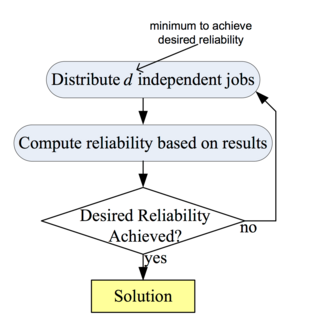
\includegraphics[width=5in]{img/Iterativeredundancyschematic}
\caption{Flowchart of Iterative Redundancy Algorithm}
\end{figure}


\item[\textbf{Fault Types}]Byzantine attacks: A Byzantine fault is one where the faulty unit continues to run but produces incorrect results and might lead to failure sometimes. 

\item[\textbf{Failure Types}]Functional failures.

\item[\textbf{Input data}] Results produced by n independent jobs that perform the same task.

\item[\textbf{Recovery actions}]The technique try to  iteratively deploy the minimum number of redundant jobs in order to achieve a consensus on a correct result.

\item[\textbf{Advantages}] Iterative redundancy is more cost effective, than traditional redundancy approaches as it creates the same level of software system reliability at a lower expense.

\item[\textbf{Disadvantages}] In iterative redundancy, the task server deploys several jobs and wait for the responses before possibly choosing to deploy more jobs. Therefore, this technique increases the latency for a particular task.

\item[\textbf{Case studies}]
The technique is implemented and tested on PlanetLab. PlanetLab is a gathering of PCs accessible as a testbed for distributed systems research.\\
\end{compactitem}


\section{SHoWA} \label{ap:Showa}
\begin{compactitem}
\item[\textbf{Title}]A Self-Healing Framework for Web-Based Applications (SH\~oWA)

\item[\textbf{Author}]Joao Paulo Magalhaes and Luis Moura Silva

\item[\textbf{Reference}]

\cite{magalhaes_showa:_2015}

\item[\textbf{Year}] 2015

\item[\textbf{Application Domain}]
Web-based applications. 

\item[\textbf{Self-Healing steps}] 
The self-healing steps involved are:Monitor, Plan, Analyse and Execute.

\item[\textbf{Technical Approach}] Statistical correlation (Spearman's rank correlation). 
%The Spearman's rank correlation coefficient (rho) measures the statistical dependence between two variables.

\item[\textbf{Basic Idea}] 
The basic idea is to collect and analyse system, application server, and application-level data, such as response time of user transactions and amount of available memory, so as to detect and pinpoint anomalies by means of statistical correlation. The performed data analysis detects changes in the server response time and analyses if those changes are correlated with a workload variation or are due to a performance anomaly. In the presence of performance anomalies, the analysis pinpoints the method calls that are more likely responsible to cause the anomaly.

\item[\textbf{Summary of approaches}] 

SH˜oWA FRAMEWORK

The SH\~oWA framework mainly works in four steps: Monitor, Analyse, Plan, and Execute. The monitor steps is executed by the sensor and data interpretation module. The analyse step is executed by the workload variation analysis, performance anomaly analysis, anomaly detector and root-clause failure analysis module. The plan step is executed by the recovery planner module and the execute step is executed by the executor and effector module. The digram below shows the different modules of the  SH\~oWA framework.

\begin{figure}[H]
\center
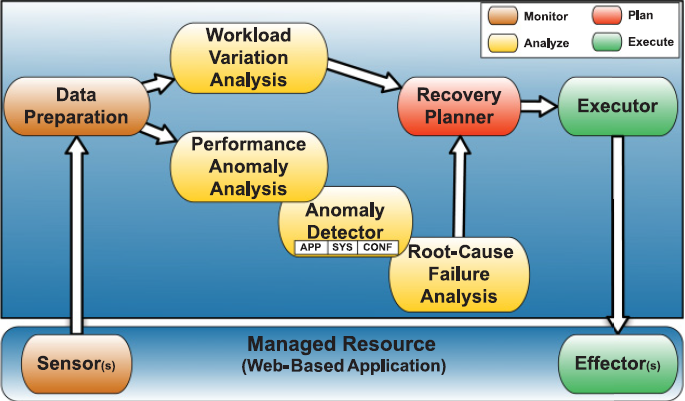
\includegraphics[width=5in]{img/selfhealingframework}
\caption{(SH\~oWA).: self healing framework}
\end{figure}

The Sensor module collects data from different system and application server parameters and measures the execution time of user transactions and application calls. The data is sent to a remote database to be prepared by the Data Preparation module. The Workload Variation Analysis and Performance Anomaly Analysis modules carry out statistical analysis to detect response time variations and to verify if the response time variations are due to workload changes or are a symptom of a performance anomaly. The Anomaly Detector module carries out statistical analysis to detect if there is any change in the system or application server parameters correlated with the performance anomaly. The Root-cause Failure Analysis module carries out statistical analysis to analyse the response time of the application calls to check if there are changes in the application, or in the invocation of remote services, that are correlated with the performance anomaly. Upon the detection and localization of performance anomalies, the recovery phase follows. The recovery phase involves the Recovery Planner module, which is responsible for selecting the recovery procedure, and the Executor module, which dispatches the recovery actions to be applied on the managed resource by the Effector module.\\

The sensor module monitors key performance indicators such as CPU load, JVM heap memory, number of open files and number of running threads. Additionally, it gathers execution time of application transactions. The data collected by the sensor module is processed by the data preparation module that associates each measurement to a specific user transactions of the monitored web application. The prepared data is then passed to the workload variation analysis and performance anomaly analysis modules to detect and pinpoint if any anomaly is present. The data analysis is based on Spearman's rank correlation coefficient represented by rho ($\rho$). The correlation coefficient is given by the equation below and  expresses how two variables are associated:

%begin{figure}[H]
%includegraphics[width=5in]{img/formulae}
%caption{Measure of statistical dependence between two %variables.}
%end{figure} 

%\rho=\frac { \sum_{ i=1} ^n(X_i-\bar{ X})(Y_i-\bar{ Y})}%%%{\sqrt{\sum_{ i=1} ^n (X_i-\bar{ X})^2 (Y_i-\bar{ Y})^2} }
%}

\begin{equation}
\rho=\frac { \sum_{ i=1} ^n(X_i-\bar{ X})(Y_i-\bar{ Y})}{\sqrt{\sum_{ i=1} ^n (X_i-\bar{ X})^2 (Y_i-\bar{ Y})^2}}
\end{equation}


where X is the sequence of the accumulated response server time per user transaction and Y is the number of user transactions processed in the same interval.If p remains stable and high across the periods of analysis, then it means that the response time is associated with the application workload (e.g., bursty workload, server queue issues). If p  decreases, then it means that one of the variables has increased or decreased while the other has remained stable or changed in an opposite direction. This dissociation corresponds to a symptom of performance anomaly (e.g. performance slowdowns from the number of user transactions processed.).Once the performance anomaly is identified by using  Spearman's rank correlation coefficient, the anomaly detector module aims to identify if there is a system or application server changes which is associated with the performance anomaly. As in the previous analyses, the anomaly detector module computes Spearman’s rank correlation coefficient $\rho$ between  the total number of user transactions processed in an interval and the accumulated value of the parameters collected by the Sensor module in the same interval. If the accumulated value of a given parameter increases and is not motivated by an increase in the number of user transactions, then the $\rho$ degree will decrease, showing that a parameter is no longer aligned with the number of requests and associating this with the performance anomaly. The data analysis in this module determines if the application is facing a performance anomaly and verifies if the anomaly is associated with changes in the parameters. If the performance anomaly is confirmed by the anomaly detection module, the root cause analysis module analyses user transactions that have only reported a performance anomaly in the previous stage. 
The root cause failure analyses module analyses the frequency of the response time of a user transaction and the response time frequency for the calls belonging to the user transaction under analysis. By applying the Spearman’s correlation analysis,this module is able to determine the list of method calls associated with the performance anomaly.

%In the current implementation, the recovery actions are procedure based and defined by human operator.In future research prospect, it is a novel idea to design the recovery procedures using the machine learning techniques.Once selected, a recovery procedure is executed by the executor module. The main job of the executor module is to execute the specific recovery action which has been triggered with respect to the specific anomaly detected.Once the recovery action has been executed, the handler is passed to the effector module which monitors and keeps track of the number of call methods that has triggered anomaly, how many
%of these are in recovery and how any of them has already been recovered.In future research prospect, it is a novel idea to design the recovery procedures using the machine learning techniques.

\item[\textbf{Fault types}]Fail-stutter fault model. 

In fail-stutter fault model, the components of a system sometimes fail and sometimes perform erratically (e.g., low performance) but are not reflected in the final results. These unexpected behaviors are defined as performance faults.

\item[\textbf{Failures types}]Performance failures.

\item[\textbf{Input data}] The input are the parameters which are collected by the sensor module. For instance user transactions, CPU time per user transactions, amount of available memory.

\item[\textbf{Recovery actions}]The output are the recovery strategies which are carried forward or executed against the particular anomalies detected.

\item[\textbf{Advantages}] In SH\~oWA sensor module the monitoring code is separated from the application code, thereby an application can be monitored without the need for manually changing its source code. With this separation, multiple applications can be monitored using the same monitoring code. The framework is generic and can be applied to any type of transactional web application. The only module that needs to be ported is the Sensor module

\item[\textbf{Disadvantages}]The ability to detect anomalies while the number of end users affected is low.
We need the source code of the application to deploy the sensor module.

\item[\textbf{Case studies}]One retail store web application and an auction web application has been used in this paper for testing the framework.
\end{compactitem}


\section{GenProg}\label{ap:GenProg}
\begin{compactitem}
\item[\textbf{Title}]GenProg: A Generic Method for Automatic Software Repair

\item[\textbf{Author}]
Claire Le Goues, ThanhVu Nguyen, Stephanie Forrest, and Westley Weimer

\item[\textbf{Reference}]  

\cite{le_goues_genprog:_2012}

\item[\textbf{Application Domain}]
Web application 

\item[\textbf{Self-Healing steps:}]. The closed loop repair system works in this way. The method adopts an IDS (intrusion-detection system) that detects the anomalies in the system. Whenever, the IDS detects an annomaly, GenProg is invoked to repair the suspicious behavior.

\item [\textbf{Technical Approach}] 

The technical approach used in this paper is genetic programming. Genetic programming (GP) is an evolutionary algorithm-based methodology which uses a set of instructions and a fitness function to measure how well a computer has performed a task.

\item[\textbf{Basic Idea}]

The basic idea is that the IDS detects an anomaly in the request and if there is an anomaly then there is an attack  and the system is stopped. Then the GenProg is invoked which takes input of the negative test case, positive test cases, and the defect and generates a variant. The variant is the automatic recovery which contains the program requirement. The variant which has the highest fitness function is considered to be the best.

A negative test case is a test case which contains the bug, if there exists a bug.

genetic program repair technique "GenProg", which uses existing test cases to automatically generate repairs.The GenProg takes an input of the set of positive test cases and the defect, searches for a program variant which retains the functionality, evaluates each variant with a user-defined fitness function and individuals with high fitness are selected for continued evolution.The variant which passes all the test cases are taken into consideration for generating the automatic final repair.

\item[\textbf{Summary of approach}] The approach implements three functions: The \textit{initialpopulation} generates the variants by using the mutual operators based on the input program and test cases. The \textit{fitness function} evaluates each variants created and chooses the best amongst them and the \textit{GenProg} iterates by selecting high fitness individuals, which are selected for continuous evolutions for the next.


The technical approach used in this paper by the author can be classified in four stages:-
\textit{Program Representation:}Each variant is represented by a pair of an abstract syntax tree   (AST)and a weighted path. The abstract syntax tree contains all the statements of the program and a weighted path contains all the statements in the program that has been assigned a weight based on the occurrence of the statement the test cases.\textit{Selection and Genetic Operators:}genProg discards individuals with fitness 0 (variants that do not compile or that pass no test cases) and places the remainder in Viable. It then uses a selection strategy to select pop size/2 members of a new generation from the previous iteration.\textit{Fitness function:}the fitness function evaluates the acceptability of a program variant. The fitness function mentioned in this paper, encodes software requirements at the test case level: negative test cases encode the fault to be repaired, while positive test cases encode functionality that cannot be sacrificed.\textit{Repair Minimization:}
the search terminates successfully when GP discovers a primary repair that passes all test cases. Due to randomness in the mutation and crossover algorithms, the primary repair typically contains at least an order-of-magnitude more changes than are necessary to repair the program, rendering the repairs difficult to inspect for correctness.


\item[\textbf{Fault Types}]Infinite loop, Segmentation fault, Remote heap buffer over flow to inject code, Remote heap buffer overflow to overwrite variables, Non overflow denial of service, Local stack buffer overflow, Integer overflow and Format string vulnerability.

\item[\textbf{Input data}] Input source code contains a failing negative test case that exercises the defect and a set of passing positive test cases that describe requirements.

\item[\textbf{Recovery actions}]The recovery action is the primary repair that passes all test cases.

\item[\textbf{Advantages}] 
The GP search space focuses genetic operations along a weighted path and takes advantage of test case coverage information, and reusing existing program statements.

\item[\textbf{Disadvantages}] GenProg relies on test cases to encode both an error to repair and important functionality. GenProg cannot repair race conditions as it is difficult to encode an error using test cases for non-deterministic properties.

\end{compactitem}

\section{QVM}\label{QVM}
\begin{compactitem}

\item[\textbf{Title}]QVM: An Efficient Runtime for Detecting Defects in Deployed Systems

\item[\textbf{Author}]
Mathew Arnold, Martin Vechev and Eran Yahav

\item[\textbf{Reference}] 

\cite{mathew_arnold_qvm:_2008}

\item[\textbf{Year}] 2008

\item[\textbf{Application Domain}]
Web services and QoS-based and AOP

\item[\textbf{Self-Healing steps}] Self-healing steps involved the following:

(i)	Finding Bugs.
The QVM monitors the correctness properties and resource leakage. The report for the bug includes the information about the allocation of the object, the object’s last state and the method invoking the object.

(ii)	Diagnosing the Cause.
The QVM provides debug information in form of type state history. For every invocation, the invocation history collects the information about the context in which the object was invoked. Hence, with the object-centric sampling, the detailed debug information is collected with low overhead.

(iii)	Developing a Fix.
QVM heap assertion leverages and checks the object for its sharing. This is done in the testing phase for fixing the problem and removal before the deployment. The problem is healed up with repetitive application of the method until the reported leak does not occur.    

\item[\textbf{Technical Approach}]

The QVM extends the VM execution engine with three main components: 
(i)	QVM interface
(ii)Overhead Manager and
(iii)QVM Clients 

\item[\textbf{Basic Idea}]  

The study is on the usability of interactive applications running with QVM. The QVM detects defects by continuously monitoring the execution of the application by checking typestate safety properties, Java assertions, and heap properties pertaining to ownership. It also provides a balanced trade-off between the cost of the monitoring process and the maintenance of sufficient accuracy for detecting defects.

\item[\textbf{Summary of approach}] Quality Virtual Machine (QVM) is a runtime environment that uses the technology and infrastructure available in a virtual machine (VM) to improve the software quality. It provides an interface that allows software monitoring clients to be executed in a controlled overhead. The goal of the system is to provide a solution having performance with low overhead and to provide maximal separation of the clients from the underlying architecture. The QVM is three tier architecture having clients at the abstract level, QVM Interface as the middleware bridging the gap among the clients and QVM’s working at the core. The input to the QVM is a user-defined overhead estimation value and the bug log report. At the initial stage the application program is connected with the QVM clients that play a major role for evaluating the performance of the system. The type state, heap probes and assertions the major clients of QVM that generate the violation report for the QVM. 

The QVM Interface (QVMI) performs three different tasks as 
1. Filtering. Filtering is done for addressing the callback requests irrespective of the working of the system. The VM provides dynamic optimization techniques to achieve an efficient implementation of the sampled profile.

2.	Property Guided Sampling. Sampling is a key mechanism for QVM that reduces the overhead. It provides dynamic analysis of the objects with its associate’s properties. With the typestate properties, the relation between the events for same object needs to be maintained.

3.	Object Centric Sampling.     At the object instances level, the objects are tracked with profile events with the objects. The tracking of objects is done at allocation time. The object sampling produces meaningful results without destroying properties associated with objects.

The OverHead Manager (OHM) known as the core of the system does the estimation of the overhead by specifying the overhead budget 5-10 \% of the deployed system. For a given overhead budget, the QVM accumulates much of information about the object. The information gathering is done by three strategies 
(i)	Monitoring. Monitoring is done by assigning a timer to the QVMI entry, exist calls and time spent on the clients. For this the QVM deploys accurate timers so that time working and existing of the threads can be tracked properly.

(ii) Sampling. With the Samplimg method QVM maintains a log for each event. A sample counter and sampleCounter Reset are added to the code for keeping the track of the event execution and abort. For severe performance degradation the QVM supports the notion of an emergency shutdown.

(iii)	Controlling. The Overhead Controller checks the QVM overhead and adjusts the sampling frequencies. The frequencies are adjusted as the budget increases or decreases periodically. Even a overhead beyond the budget can cause an emergency shutdown.
However, with early tracking of the objects, early resource release can be done for increasing the performance. 

\begin{figure}[H]
\center
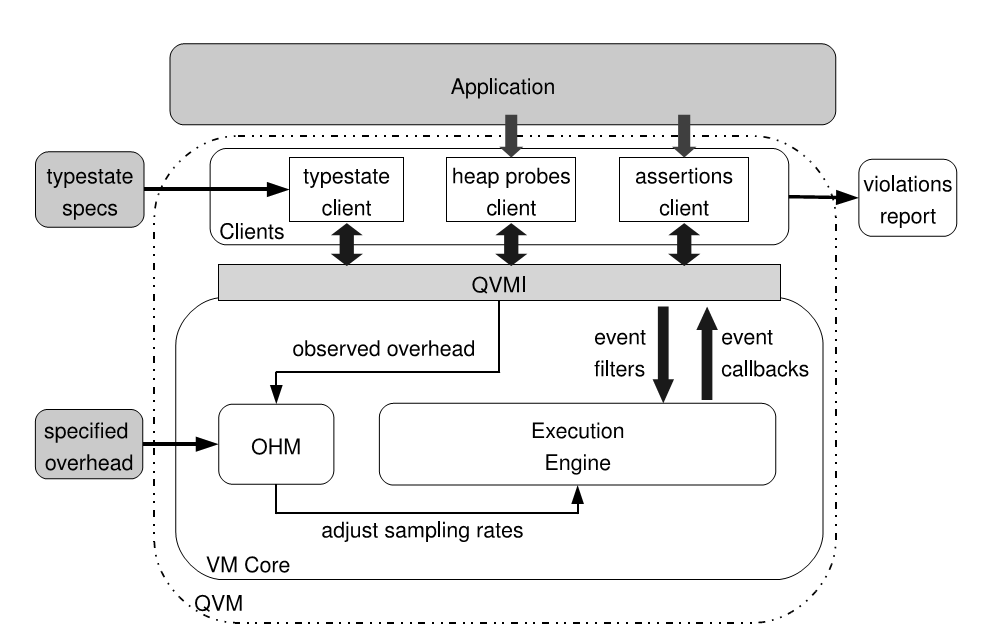
\includegraphics[width=5in]{img/qvm}
\caption{Overall architecture of QVM.}
\end{figure}

\item[\textbf{Fault Types}]
(i)	Typestates assertions
(ii)	Resource Leakage
(iii)	Java assertions
 
\item[\textbf{Failure Types}]

(i)	Performance Degradation

\item[\textbf{Input data}] 

(ii)	Overhead estimation
(iii)	Bug log file


\item[\textbf{Recovery actions}]

(i)	Resource utilization
(ii)Leverage heap probe 


\item[\textbf{Advantages}] 

(i)	High-performance and low overhead
(ii)	Maximal separation of analysis clients from virtual machine (VM)
(iii)	Runtime access for the clients allows for utilizing information
(iv)	The access to dynamic optimizer (JIT) ensures to critical code paths are well optimized
(v)	The efficient dynamic updating of VM can be upgraded with the application of the advance techniques such as code patching and on-stack replacement.  
(vi)	The deployment becomes easier as the required features are installed in the VM.


\item[\textbf{Disadvantages}] 

(i)	Quality service implementation on VM makes them non-portable
(ii)	The users of the system are meant specific to VM version

\item[\textbf{Case study}] 

(i)	The QVM run on eclipse
(ii)	The QVM run on development version of a large scale IBM product. 

\end{compactitem}




